
\documentclass[11pt, a4paper]{article}
%\usepackage{proj1}
\usepackage{natbib}
\usepackage{fancyhdr}  
\usepackage{subcaption}
\usepackage{caption}
\usepackage{graphicx}
\usepackage{numprint}
\usepackage{multirow}
\linespread{1.25} 
\setlength{\parindent}{0cm}
\graphicspath{{Images/}}
\usepackage{hyperref}
\usepackage{amsmath}
\usepackage{amsfonts}
\usepackage{amssymb}
\usepackage{amsthm}
\usepackage{mathtools}
\usepackage{commath}
\usepackage{bbm}

%\usepackage[sc,osf]{mathpazo}
\usepackage{subcaption}
\usepackage[a4paper, top=1in, left=1.0in, right=1.0in, bottom=1in, includehead, includefoot]{geometry} %Usually have top as 1in

\usepackage{listings}
\usepackage{color} %red, green, blue, yellow, cyan, magenta, black, white
\definecolor{mygreen}{RGB}{28,172,0} % color values Red, Green, Blue
\definecolor{mylilas}{RGB}{170,55,241}


\hypersetup{colorlinks,linkcolor={black},citecolor={blue},urlcolor={black}}
\usepackage{color}
\urlstyle{same}


\theoremstyle{definition}
\newtheorem{definition}{Definition}[section]

\newcommand{\adja}{q_a}
\newcommand{\adjb}{q_b}
\newcommand{\adjaB}{q_{a,\partial \Omega}}
\newcommand{\adjbB}{q_{b,\partial \Omega}}
\newcommand{\adjB}{q_{\partial \Omega}}
\newcommand{\Adja}{\mathbf{p}}
\newcommand{\Adjb}{q}
\newcommand{\adj}{q}
\newcommand{\Adjc}{{q}_{\partial \Omega}}
\newcommand{\ra}{\rho_a}
\newcommand{\rb}{\rho_b}
\newcommand{\w}{\mathbf{w}}
\newcommand{\x}{\mathbf{x}}
\newcommand{\f}{\mathbf{f}}
\newcommand{\ve}{\mathbf{v}}
\newcommand{\n}{\mathbf{n}}
\newcommand{\h}{\mathbf{h}}
\newcommand{\K}{\mathbf{K}}
\newcommand{\hr}{\widehat \rho}
\newcommand{\jf}{\mathbf j}

\DeclareMathOperator{\sgn}{sgn}
\DeclareMathOperator{\Grad}{Grad}
\DeclareMathOperator{\Div}{Div}
\DeclareMathOperator{\Lap}{Lap}
%	\begin{figure}[h]
%		\centering
%		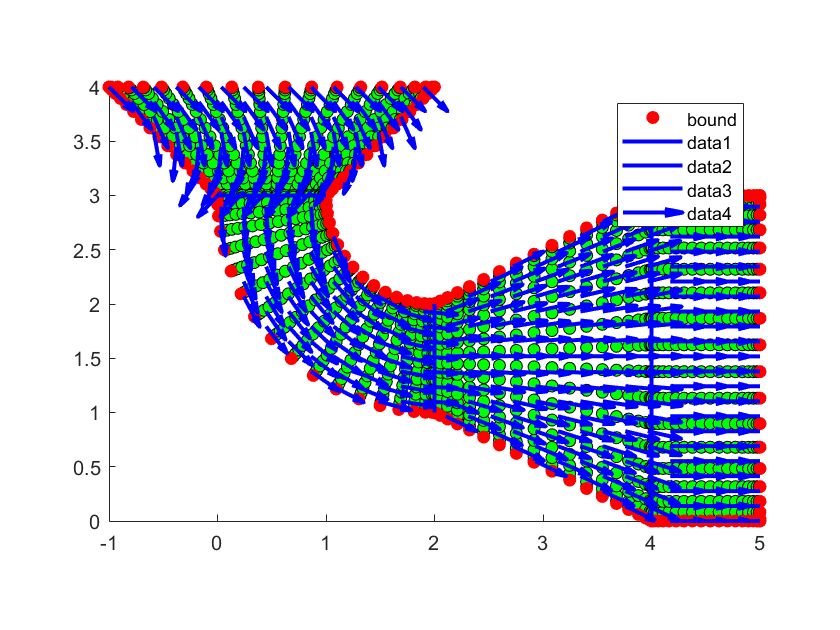
\includegraphics[scale=0.35]{F1.png}
%		\caption{Forward $\rho$ for $a = 0.01$} 
%		\label{F1}
%	\end{figure}

\begin{document}
Annual Review (in particular structure).\\
issues with Datastorage
\section{Newton-Krylov}
Second example works, has absolute value $10^{-5}$ and relative error $10^{-3}$ for $\beta = 10^{-3}$. For $\beta = 10$ we are at $10^{-6}$ absolute and $10^{-4}$ relative error as for all other problems.
My suspicion was that the target is too concentrated, so we get advection dominance. I smoothed out the target to be
\begin{align*}
	\hr = (1-t)0.25 + t(1/2.1445)\exp(-((x1+0.2)^2 + (x2+0.2)^2))
\end{align*},
where the exponential prefactor is reduced from $3$ to $1$ and the normalising constant is adjusted appropriately.
This results in $10^{-6}$ and $10^{-4}$ error for $\beta = 10^{-3}$, which supports my hypothesis from above. It would be interesting to see whether it is Newton-Krylov or Fixed Point that's inaccurate by comparing to fsolve.

\section{3D Convolution}
The below code shows the 3D Convolution implementation.
%\lstset{language=Matlab}  %  M1 = I;  M2 = I; at end of line with f, g
\begin{lstlisting}[frame=single]  % Start your code-block
    
    function M_conv = ComputeConvolutionMatrix(this,f,saveBool)
	
		if(nargin(f)==1)
			useDistance = true;
		else
			useDistance = false;
		end
	
		N1  = this.N1;  N2  = this.N2;  N3  = this.N3;
		Pts = this.Pts;
		Int = this.Int;  % 1 x N1*N2
		
		if(useDistance)
			fPTemp = f(GetDistance(this,Pts.y1_kv,...
			Pts.y2_kv,Pts.y3_kv));
		else
			fPTemp = f(Pts.y1_kv,Pts.y2_kv,Pts.y3_kv);
		end
		
		fDim = size(fPTemp);
		
		nElts = prod(fDim(2:end));
		
		IntT = Int.';  % N1*N2 x 1
		
		IntT = IntT(:,ones(1,nElts)); % N1*N2 x nElts
		IntT = reshape(IntT,fDim);    % size(f)
		
		M_conv = zeros([N1*N2*N3,N1*N2*N3,fDim(2:end)]);
		
		Mmask = repmat({':'},[1,fDim]);
		
		for i=1:(N1*N2*N3) 
	    	if(useDistance)
		   fP = f(GetDistance(this,Pts.y1_kv(i) - Pts.y1_kv,...
                     Pts.y2_kv(i) - Pts.y2_kv,...
  		             Pts.y3_kv(i) - Pts.y3_kv));
		 else
		   fP = f(Pts.y1_kv(i) - Pts.y1_kv,...
				Pts.y2_kv(i) - Pts.y2_kv,...
				Pts.y3_kv(i) - Pts.y3_kv);
		 end
		Mmask{1} = i;
		M_conv(Mmask{:}) = IntT.*fP;
		end
		M_conv(isnan(M_conv)) = 0;
		
		if((nargin >= 3) && islogical(saveBool) && saveBool)
			this.Conv = M_conv;
		end
	
	end   
	
	function d  = GetDistance(this,pts_y1,pts_y2,pts_y3)             
		if(nargin == 2)
			pts_y3 = pts_y1.y3_kv;
			pts_y2 = pts_y1.y2_kv;
			pts_y1 = pts_y1.y1_kv;
		end
		
		%ptsCart = GetCartPts(this,pts_y1,pts_y2,pts_y3);
		%d       = sqrt(ptsCart.y1_kv.^2 + ptsCart.y2_kv.^2); 
		d       = sqrt(pts_y1.^2 + pts_y2.^2 + pts_y3.^2);
	end
\end{lstlisting}
\subsection{Testing Convolution}
We compute the convolution
\begin{align*}
	n * \chi (x) = \int_\Omega \chi(x - y) n(y) dy.
\end{align*}
In a first example we have
\begin{align*}
	n(\vec y) &= \cos(y_1),\\
	\chi(\vec y) &= \sin(y_1 + y_2 + y_3),
\end{align*}
with the exact solution
\begin{align*}
	n * \chi (\vec x) &= 0.5 \sin(0.5) \left(-2\sin(0.5)\cos( 1 - c ) + 2 \sin(0.5)\cos(3 - c) - 4\sin(0.5)\sin(1 - c) \right),\\
	c &= x_1 + x_2 + x_3,
\end{align*}
in $[0,1]^2$. With $N = 10$, we have an error of $2.7412 \times 10^{-11}$.
\\
\\
Next we test 
\begin{align*}
	n(\vec y) &= y_1 y_2 y_3,\\
	\chi(\vec y) &= exp(-|\vec y|^2),
\end{align*}
with the exact solution
\begin{align*}
	T_1 &= (1/2)(\exp(-x_1^2) + \sqrt\pi x_1(erf(1 - x_1) + erf(x_1)) - \exp( - (x_1 - 1)^2)),\\
	T_2 &= (1/2)(\exp(-x_2^2) + \sqrt\pi x_2(erf(2 - x_2) + erf(x_2)) - \exp( - (x_2 - 2)^2)),\\
	T_3 &= (1/2)(\exp(-x_3^2) + \sqrt\pi x_3(erf(3 - x_3) + erf(x_3)) - \exp( - (x_3 - 3)^2)),\\
	n * \chi (\vec x) &= T_1 T_2 T_3,
\end{align*}
on $[0,1] \times [0,2] \times [0,3]$.
For $N = 10$ the error is $8.2056 \times 10^{-5}$. For $N = 15$ it reduces to $5.8809 \times 10^{-8}$ and for $N = 20$ we get $6.6143 \times 10^{-11}$.
\\
\\
Finally we consider
\begin{align*}
	n(\vec y) &=(\sin(\pi y_1)^2)(\sin(\pi y_2)^2)(\sin(\pi y_3)^2)\\\
	\chi(\vec y) &= y_1 y_2 y_3\
\end{align*}
with the exact solution
\begin{align*}
	n * \chi (\vec x) &= (1/4)(2y_1 - 1)(y_2 - 1)(3/4)(2y_3 - 3),
\end{align*}
on $[0,1] \times [0,2] \times [0,3]$.
For $N = 10$ we get an error of $0.0015$ and for $N = 20$ it reduces to $7.7335 \times 10^{-8}$. For $N = 25$ we get $1.0006 \times 10^{-11}$.
The errors are measured in the absolute standard Matlab norm.
\section{Curl free control}	
We consider
\begin{align*}
	&\min_{\rho, \w} \frac{1}{2}\int_0^T \int_\Omega \left(\rho - \hr\right)^2 d\x dt + \frac{\beta}{2}\int_0^T \int_\Omega \w^2 d\x dt + \frac{\eta}{2}\int_0^T \int_\Omega \left(\nabla \times \w \right)^2 d\x dt\\
	&\text{subject to:}\\
	& \frac{\partial \rho}{\partial t} = \nabla^2 \rho - \nabla \cdot \left(\rho \w\right)\\
	& \frac{\partial \rho}{\partial n} - \rho \w \cdot \n = 0
\end{align*}
We know that in two dimensions
\begin{align*}
    \nabla \times \w = \frac{\partial w_2}{\partial x_1}  - \frac{\partial w_1}{\partial x_2}.
\end{align*}
More importantly, we know that
\begin{align}\label{eqn:CurlRel}
	\nabla \times \w = \nabla \cdot  \w_\bot,
\end{align}
where $\w_\bot = (w_2 , -w_1)$, the result of a rotation of $\w$ by $\pi/2$.
Then the Lagrangian is
\begin{align*}
	\mathcal L (\rho, \w ,q_1, q_2) =& \frac{1}{2}\int_0^T \int_\Omega \left(\rho - \hr\right)^2 d\x dt + \frac{\beta}{2}\int_0^T \int_\Omega \w^2 d\x dt + \frac{\eta}{2}\int_0^T \int_\Omega \left(\nabla \cdot  \w_\bot \right)^2 d\x dt\\
	&- \int_0^T \int_\Omega q_1 \left(\frac{\partial \rho}{\partial t} - \nabla^2 \rho + \nabla \cdot \left(\rho \w\right) \right) d \x dt \\
	&- \int_0^T \int_{\partial \Omega} q_2\left(\frac{\partial \rho}{\partial n} - \rho \w \cdot \n \right) d\x dt.
\end{align*}
Then, since we know that $q_1 = q_2$, we get
\begin{align*}
	\mathcal L (\rho, \w ,q) =& \frac{1}{2}\int_0^T \int_\Omega \left(\rho - \hr\right)^2 d\x dt + \frac{\beta}{2}\int_0^T \int_\Omega \w^2 d\x dt + \frac{\eta}{2}\int_0^T \int_\Omega \left(\nabla \cdot  \w_\bot\right)^2 d\x dt\\
	&- \int_0^T \int_\Omega -\rho\frac{\partial q}{\partial t} - \rho \nabla^2 q - \nabla q \cdot \left(\rho \w\right) d \x dt  - \int_\Omega q(T) \rho(T) - q(0) \rho(0) d\x\\
	&- \int_0^T \int_{\partial \Omega}  - \rho \nabla q \cdot \n  d\x dt.
\end{align*}
For the adjoint equation, we find the usual results.
We take the derivative with respect to $\w$
\begin{align*}
	\mathcal L_\w(\rho, \w, q)h &= \int_0^T \int_\Omega \beta \w \cdot  \h + \rho \nabla q \cdot \h + \eta \left(\nabla \cdot  \h_\bot\right) \left(\nabla \cdot  \w_\bot\right)d\x dt.
\end{align*}
Then we integrate by parts (or divergence theorem) to get
\begin{align*}
	\mathcal L_\w(\rho, \w, q)h &= \int_0^T \int_\Omega \beta \w \cdot  \h + \rho \nabla q \cdot \h - \eta \nabla\left(\nabla \cdot  \w_\bot\right)  \cdot \h_\bot d\x dt + \int_0^T \int_{\partial \Omega} \eta \left(\nabla \cdot  \w_\bot\right) \h_\bot \cdot \n d \x dt.
\end{align*}
Finally we need to rewrite the equations in terms of $\h$. We note that 
\begin{align*}
	\begin{pmatrix}
		0 & 1\\
		-1 & 0
	\end{pmatrix} 
\h
= 
\h_\bot.
\end{align*}
Furthermore,
\begin{align*}
	\begin{pmatrix}
		0 & -1\\
		1 & 0
	\end{pmatrix} 
	\n \cdot \h
	= 
	\h_\bot \cdot \n.
\end{align*}
Replacing these in the Lagrangian gives
\begin{align*}
	\mathcal L_\w(\rho, \w, q)h &= \int_0^T \int_\Omega \beta \w \cdot  \h + \rho \nabla q \cdot \h - \eta 	\begin{pmatrix}
		0 & -1\\
		1 & 0
	\end{pmatrix} \nabla\left(\nabla \cdot  \w_\bot\right)  \cdot
	\h d\x dt \\
	&+ \int_0^T \int_{\partial \Omega} \eta \left(\nabla \cdot  \w_\bot\right) \begin{pmatrix}
		0 & -1\\
		1 & 0
	\end{pmatrix} 
	\n \cdot \h d \x dt.
\end{align*}
Finally, using \eqref{eqn:CurlRel} we get
\begin{align*}
	\mathcal L_\w(\rho, \w, q)h &= \int_0^T \int_\Omega \beta \w \cdot  \h + \rho \nabla q \cdot \h - \eta 	\begin{pmatrix}
		0 & -1\\
		1 & 0
	\end{pmatrix} \nabla\left(\nabla \times  \w\right)  \cdot
	\h d\x dt \\
	&+ \int_0^T \int_{\partial \Omega} \eta \left(\nabla \times \w\right) \begin{pmatrix}
		0 & -1\\
		1 & 0
	\end{pmatrix} 
	\n \cdot \h d \x dt.
\end{align*}
Since this holds for all admissible $\h$ we get the gradient equation
\begin{align*}
	 \beta \w  + \rho \nabla q - \eta 	\begin{pmatrix}
	 	0 & -1\\
	 	1 & 0
	 \end{pmatrix} \nabla\left(\nabla \times  \w\right) &= 0\quad \text{in} \quad \Omega\\
	\eta \left(\nabla \times \w\right) \begin{pmatrix}
		0 & -1\\
		1 & 0
	\end{pmatrix} 
	\n &= 0 \quad \text{on} \quad \partial \Omega.
\end{align*}
In component form this is 

\begin{align*}
	\beta w_1 + \rho \frac{\partial q}{\partial x_1} - \eta \left(\frac{\partial^2 w_1}{\partial x_2^2} - \frac{\partial^2 w_2}{\partial x_1 \partial x_2} \right) &= 0\quad \text{in} \quad \Omega\\
	-\eta \left(\frac{\partial w_2}{\partial x_1} - \frac{\partial w_1}{\partial x_2} \right)n_2 &= 0 \quad \text{on} \quad \partial \Omega.
\end{align*}
and
\begin{align*}
	\beta w_2 + \rho \frac{\partial q}{\partial x_2} - \eta \left( \frac{\partial^2 w_2}{ \partial x_1^2} -\frac{\partial^2 w_1}{\partial x_1 \partial x_2}\right) &= 0\quad \text{in} \quad \Omega\\
	\eta \left(\frac{\partial w_2}{\partial x_1} - \frac{\partial w_1}{\partial x_2} \right)n_1 &= 0 \quad \text{on} \quad \partial \Omega.
\end{align*}


\end{document}